%!TEX root = ../report.tex
\section{Taktik}

\subsection{Begriffe \& Systematik}
\begin{description}
  \item[Taktik] ist ein System von Handlungsplänen und Entscheidungsalternativen, das Trainings- und Wettkampfverhalten so zu regulieren gestattet, dass ein optimaler sportlicher Erfolg möglich wird.
  \item[Strategie] ist über längere Zeit gesehene Taktik.
  \item[Taktisches Verhalten] bedeutet eine Situation mit einer Handlung zu beantworten
  \item[Taktisch entscheiden] bedeutet in einer Situation aus einer Menge aus Alternativen einen Handlungsplan auswählen. Es existieren verschiedene Kopplungsmodelle dieses Auswahlverfahrens: Feste Assoziation (eine Situation impliziert genau eine Handlung), Auswahl aus Alternativen (eine Situation kann eine Gruppe von Handlungen implizieren), Vorsatzhandlungen (es existiert nur eine Handlungsalternative).
\end{description}
\begin{figure}[H]
  \begin{flushleft}
    \textbf{Systematisierung nach Zeit}
  \end{flushleft}
  \centering
  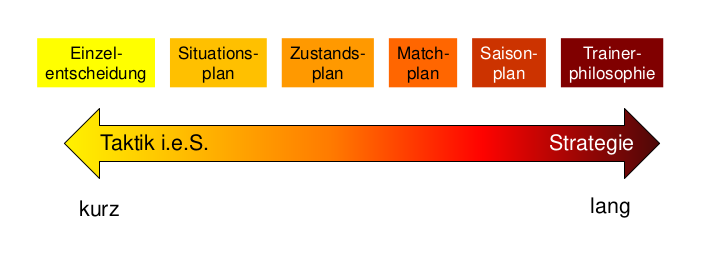
\includegraphics[width=.7\textwidth]{pictures/taktik_systematisierung.png}
  \caption{Systematisierung von Taktik nach Zeit}
\end{figure}
\paragraph{Systematisierung nach \# beteiligter Spieler} Taktik kann abhängig von der Anzahl der Spieler eingeteilt werden. Teilbereiche sind dann Mannschaftstaktik, Gruppentaktik und Individualtaktik.
\paragraph{Systematisierung nach Spielsituation} Mögliche Varianten sind Standardsituation, Offensivtaktik, Defensivtaktik, Übergangsphasen
\paragraph{Systematisierung nach Trainingszielen}
\begin{itemize}
  \item Taktische Kenntnisse: Wissensbestände, deklaratives Wissen
  \item Taktische Fähigkeiten: Situationsübergreifende taktische Handlungskompetenz: Wahrnehmung, Entscheidung, Ausführung
  \item Taktische Fertigkeiten: Angemessene und erfolgreiche Antworthandlungen (Individuell, teilkollektiv und kollektiv)
\end{itemize}
\paragraph{Taktische Handlungsphasen (nach Heckhausen)}
\begin{enumerate}
  \item Prädezisionale Phase: Wählen/ Entscheiden
  \item Präaktionale Phase: Planen/ Abschirmen
  \item Aktionale Phase: Ausführen
  \item Postaktionale Phase: Vergleichen/ Bewerten
\end{enumerate}
\begin{figure}[H]
  \begin{flushleft}
    \textbf{Phasenstruktur taktischen Handelns (nach Mahlo)}
  \end{flushleft}
  \centering
  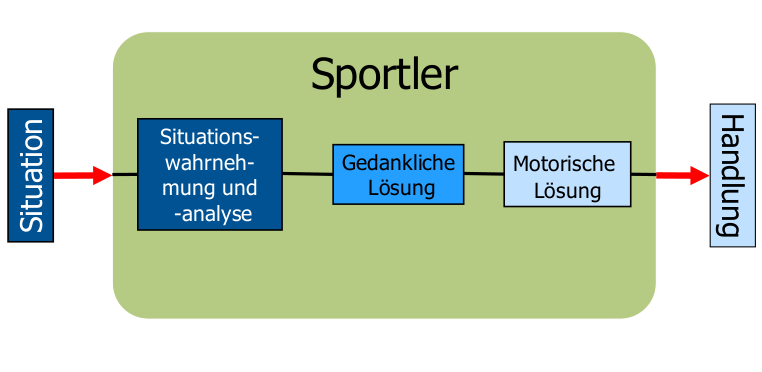
\includegraphics[width=.7\textwidth]{pictures/taktik_phasenstruktur_des_handelns.png}
\end{figure}
Probleme dieses Ansatzes:
\begin{itemize}
  \item Werden die Phasen vollständig durchlaufen?
  \item Werden die Phasen nacheinander druchlaufen?
  \item Entscheidungen werden bewusst getroffen
\end{itemize}
\paragraph{Fehlerquellen bei taktischen Entscheidungen} Taktische Fehlentscheidungen können durch alle 3 Phasen enstehen. Falsche Situationswahrnehmung und -analyse (sensorische Probleme), Inkorrekte gedankliche Lösungen (Wahl der falschen Alternative, Menge an Vorerfahrung, akt. Einflüsse) und eine mangelnde motorische Umsetzung (Fehleinschätzung der Fähigkeiten, situative Umstände)
\paragraph{Entscheidungsmodelle der Psychologie}
\begin{itemize}
  \item Zufallsentscheidung
  \item Heuristische Entscheidung
  \item Rational-Choice Entscheidung: viele Theorien, z.B.\ Erwartungs-mal-Wert-Therie (Probleme: alle Alternativen, Werte \& Wahrscheinlichkeiten bekannt?)
\end{itemize}
\paragraph{Aktuelle Theorien - Top-down \& Bottom-up Prozesse}
\begin{description}
  \item[Top-down Prozesse] Kognitionsgesteuerte, verbalisierbare Erwartungs- und Zielbildungsprozesse (Wenn A dann B)
  \item[Bottom-up Prozesse] Wahrnehmungs- gesteuerte, nicht verbalisierbare Wahrnehmungs- Handlungsprozesse. (Reaktionen)
\end{description}
Mögliche Zusammenspiele der beiden Prozesse:\\
\begin{minipage}{0.1\textwidth}
  
\includegraphics[width=\textwidth]{pictures/taktik_top-down_bottom-up.png}
\end{minipage}
\begin{minipage}{0.9\textwidth}
  \begin{itemize}
    \item Selektion: Nur je ein Typ aktiv (Vorsatzhandlungen)
    \item Konkurrenz: 1 Typ dominiert, i.d.R.\ Top-down (einfache Situationen)
    \item Kooperation: beide in gleiche Richtung (komplexe Situationen)
    \item Korrektur: Wahrnehmung korrigiert Entscheidung
  \end{itemize}
\end{minipage}
Top-down Prozesse sind explizit lehrbar, Bottom-up nicht/nur implizit. Lehren von Top-down Prozessen beinhaltet taktisches Wissen, Spielsysteme, Standardsituationen und Vorsatzhandlungen. Implizites Botto-up Training beinhaltet das Verhalten im Raum, das Erkennen von Optionen, Lesen des Gegners und die Lösung von Situationen.

\subsection{Determinanten}
\begin{figure}[H]
  \centering
  \begin{subfigure}{.45\textwidth}
    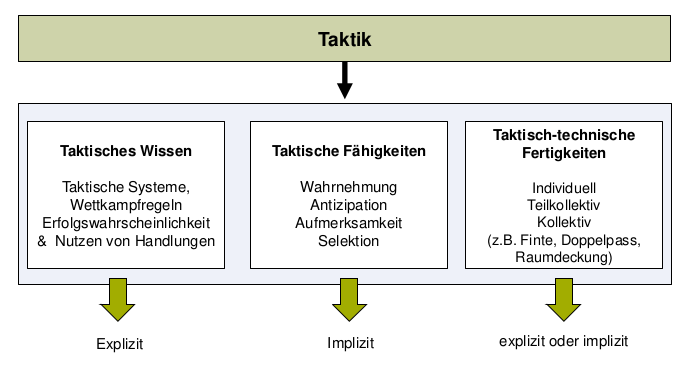
\includegraphics[width=\textwidth]{pictures/taktik_determinanten.png}
    \caption{Allgemeine Determinanten}
  \end{subfigure}
  \begin{subfigure}{.45\textwidth}
    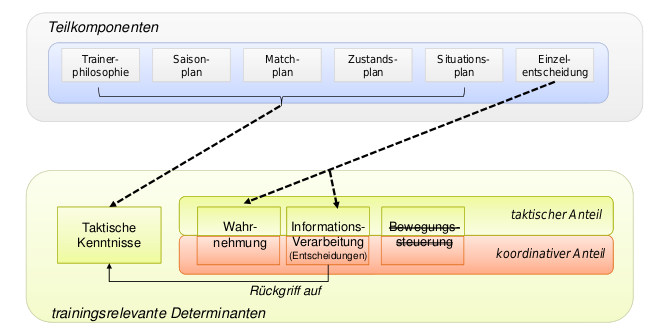
\includegraphics[width=\textwidth]{pictures/taktik_determinanten_trainingsrelevant.png}
    \caption{Trainingsrelevante Determinanten}
  \end{subfigure}
\end{figure}

\subsection{Trainingsinhalte}
Taktische Kenntnisse $\rightarrow$ Wissensvermittlung\\
Realisation von geplanten Spielzügen $\rightarrow$ Abstimmung zwischen Mannschafften\\
Situatives Lösen von offenen Situationen $\rightarrow$ Korrektheit und Schnelligkeit der taktischen Entscheidung
\paragraph{Rolle des Bewusstseins} Bewusstseinspflichtige Inhalte (z.B.\ Regeln) und bewusstseinsfähige Inhalte (z.B.\ Erfolgswahrscheinlichkeit von Handlungen) bilden die taktischen Kenntisse. Zusätzlich gibt es noch nicht-bewusstseinsfähige Inhalte (z.B.\ schnelle Entscheidungen) die nicht zur Taktik zählen.
\paragraph{Vermittlungskonzepte}
\begin{itemize}
  \item Explizit/Intentional: Systematisches Lernen\\
    Beispielhafte Übungsreihe:\\
    \begin{tabular}{m{0.4\textwidth} | m{0.4\textwidth}}
      Stufen & Inhalt \\ \hline
      Isoliertes Üben der Handlungsalternative A & Üben mit fest vorgegebenem Verhalten A \\ \hline
      Isoliertes Üben der Handlungsalternative B & Üben mit fest vorgegebenem Verhalten B \\ \hline
      Entscheidungstraining\newline Handlungsalternative A oder B? & Üben, bei dem überwiegend Abwehrverhalten A \newline gezeigt wird und nur selten Abwehrverhalten B \\ \hline
      Handlungsalternative B oder A? & Üben, bei dem überwiegend Abwehrverhalten B\newline
      gezeigt wird und nur selten Abwehrverhalten A \\ \hline
      Isoliertes Übender Handlungsalternative C & Üben mit fest vorgegebenem Verhalten C \\ \hline
      Entscheidungstraining & \ldots \\ \hline
      Wettkampfnahes Spieltraining/Anwendung im Wettspiel & Üben mit nicht eingeschränkten Gegnerverhalten \\
    \end{tabular}
  \item Implizit/Inzidentell: Unbewusstes Lernen am Einzellfall (mit Vorgabe der Rahmenbedingungen.\\
    Menschen lernen Dinge unbewusst ohne explizite Erklärung. Dafür wird vor Allem intrinsische Motivation genötigt, ansonsten kein Fortschritt.
\end{itemize}
\textbf{Theorie der antizipativen Verhaltenskontrolle nach Hoffmann}\newline
  \begin{minipage}{.5\textwidth}
  In einer Ausgangsbedingung ($S_{Augs}$) werden Konsequenzen ($K_{Ant}$) des eignen Handelns (R) antizipiert und mit real eingetroffener Konsequenz ($K_{Real}$) verglichen.
  Bei Gleichheit wird die Assoziation verstärkt, ansonsten findet eine Neubewertung der Ausgangssituation statt.\\
  Lernen besteht darin, die Differenzen durch Restrukturierung der Äquivalezklassen zu minimieren.
  Die AVK (d.h.\ die Einteilung in die einzelnen Teilabschnitte) ist anwendbar für den ganzen Bereich von Bottom-up zu Top-down Prozessen.
  \end{minipage}
  \begin{minipage}{.5\textwidth}
    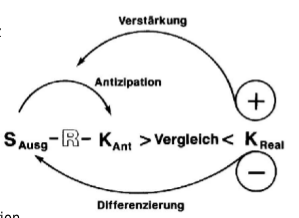
\includegraphics[width=\textwidth]{pictures/taktik_avk.png}
  \end{minipage}

\subsection{Trainingsmethoden}
\paragraph{Grundsätze}
\begin{itemize}
  \item Ähnliche, homogene Situationen schaffen und Assoziationen mehrfach bestätigen
  \item Verhaltensziele nicht IMMER erreichen, zur Differenzierung von Situationen
  \item Komplexitätssteigerung für Grenzfälle
  \item Explizite Hinweise, z.B.\ Anzeigen von Handlungsmöglichkeiten
  \item Realistische Entscheidungsalternativen
\end{itemize}
\begin{figure}[H]
  \begin{flushleft}
    \textbf{Abgrenzung Schelligkeits-, Koordinations- \& Taktiktraining}\\
  \end{flushleft}
  \centering
  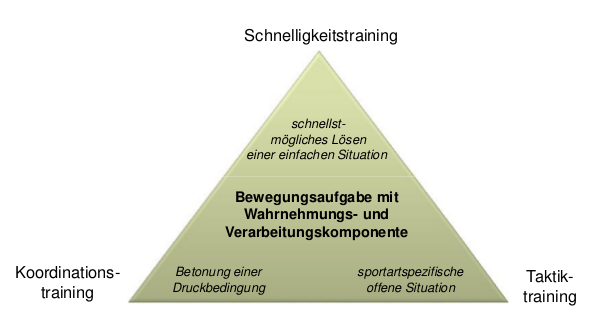
\includegraphics[width=.7\textwidth]{pictures/taktik_training_abgrenzung.png}
\end{figure}

\subsection{Anwendung}
\begin{tabular}{p{.3\textwidth} | p{.3\textwidth} | p{.3\textwidth}}
  & Pro & Contra \\ \hline 
  Explizit & 
    \begin{itemize}[noitemsep,nolistsep]
      \item gezielt, systematisch
      \item kann sofort wirken
    \end{itemize} &
    \begin{itemize}[noitemsep,nolistsep]
      \item Explosion von Regeln
      \item Verlust von Detailinformationen
      \item gebunden an Aufmerksamkeit, vergessensanfällig
      \item behindert Einsicht, Kreativität
    \end{itemize}\\ \hline
  Implizit & 
    \begin{itemize}[noitemsep,nolistsep]
      \item Praxisevidenz
      \item Intrinsische Motivation
    \end{itemize} & 
    \begin{itemize}[noitemsep,nolistsep]
      \item Erfolg nicht unmittelbar herbeiführbar.
      \item langsam
      \item schlechte Belegbarkeit
    \end{itemize}\\ \hline
\end{tabular}

\subsection{Diagnostik}
\paragraph{Spielanalyze} ist eine analytische, zielgerichtet Beschreibung und Interpretation des Verhaltens im Sportspiel zum Zweck der Leistungsdiagnose.
Es gibt 2 methodische Grundtypen:
\begin{description}
  \item[Quantitativ] Verhalten wird auf ein Beobachtungssystem abgebildet, die Ergebnisse sind konkrete Zahlen.
    \begin{itemize}
      \item Beobachtungssystem: Struktur der zu erhebenden Daten in einem Modell
      \item Beobachtungseinheit: Elementarereignis (z.B.\ Ballkontakte)
      \item Beobachtungsmerkmal: Eigenschaft einer Beobachtungseinheit (z.B.\ Spieler, Annahmequalität)
      \item Merkmalsausprägungen: Arten, wie ein Merkmal auftreten kann (z.B.\ gut, schlecht, 42cm)
      \item Typen von Ausprägungen (z.B.\ Nominalmerkmale, Ganzzahl)
    \end{itemize}
  \item[Qualitativ] Geschehen wird beobachtet mit eigener Expertise verglichen, die Ergebnisse sind Einschätzungen und Interpretationen.
\end{description}

\subsection{Zusammenfassung}
